\documentclass[12pt]{beamer}
\usetheme{default}
\usecolortheme{crane}
%\usetheme{Madrid}

\usepackage[utf8x]{inputenc}
\usepackage[T1]{fontenc}
\usepackage[slovak]{babel}
\usepackage{ucs}
\usepackage{amsmath}
\usepackage{graphicx}
\usepackage{array}
\usepackage{amsmath, amssymb}
\usepackage{hyperref, url}
%\usepackage[inline]{asymptote}

%\setbeamersize{text margin left=1pt,text margin right=1pt}
\setbeamertemplate{footline}[frame number]
\beamertemplatenavigationsymbolsempty

\let\o=\vee
\let\a=\wedge
\let\bigo=\bigvee
\let\biga=\bigwedge

\title{Relačný model a úvod do SQL}
\author{Ján Mazák}
\institute{FMFI UK Bratislava}
\date{}
%\date % (optional)
%{23. 9. 2019}

% database-related stuff
\DeclareMathOperator{\join}{\bowtie}
\DeclareMathOperator{\antijoin}{\rhd}

\DeclareMathOperator{\COUNT}{\textrm{COUNT}}
\DeclareMathOperator{\SUM}{\textrm{SUM}}
\DeclareMathOperator{\MAX}{\textrm{MAX}}


\DeclareMathOperator{\osoba}{osoba}
\DeclareMathOperator{\firma}{firma}
\DeclareMathOperator{\vlastni}{vlastni}
\DeclareMathOperator{\ponuka}{ponuka}
\DeclareMathOperator{\chce}{chce}
\DeclareMathOperator{\lubi}{lubi}
\DeclareMathOperator{\capuje}{capuje}
\DeclareMathOperator{\navstivil}{navstivil}
\DeclareMathOperator{\vypil}{vypil}
\DeclareMathOperator{\answer}{answer}


\begin{document}

\frame{\titlepage}

\begin{frame}{Relačný model}
Databáza pozostáva z tabuliek (\alert{relácií}).\\[3mm]

Stĺpce --- \alert{atribúty}; každý má doménu (množinu povolených hodnôt, čiže dátový typ prípadne zúžený dodatočnými obmedzeniami). Určené pomenovaním alebo pozíciou.\\[3mm]

Riadky --- \alert{záznamy} (records, rows, tuples, n-tice).
\end{frame}

\begin{frame}[fragile]{Relačný model}
\begin{verbatim}
CREATE TABLE employees (
    id INTEGER PRIMARY KEY,
    lastName TEXT NOT NULL,
    firstName VARCHAR(255),
    age INTEGER CHECK (age >= 18)
);
\end{verbatim}
\end{frame}

\begin{frame}{Relačný model}
Reláciu možno vnímať ako predikát alebo ako (multi)množinu záznamov.\\[3mm]

V bežných DBMS sa relácia chápe ako multimnožina:
\begin{itemize}
\item na poradí riadkov nezáleží;
\item riadky v tabuľke sa môžu opakovať.
\end{itemize}

Odstránenie duplikátnych záznamov z výsledku dotazu:\\
SELECT DISTINCT x, y FROM ...
\end{frame}

\begin{frame}{NULL}
\begin{itemize}
\item Špeciálna hodnota \alert{NULL} zodpovedá neznámej hodnote.
\item Trojhodnotová logika, napr. `NULL OR FALSE` je NULL.
\item Test, či je hodnota NULL: `x IS NULL`, `x IS NOT NULL`
\item Pri vytváraní tabuľky možno NULL zakázať.
Inak treba starostlivo uvažovať, ako ovplyvní operátory a agregačné funkcie (napr. priemer hodnôt v stĺpci).
Nehádajte, použite dokumentáciu.
\end{itemize}
\end{frame}

\begin{frame}[fragile]{Dotazy v SQL}
Základná štruktúra:
\begin{verbatim}
SELECT attr1 AS a1, attr2 AS a2
FROM table AS t
WHERE t.a2 > 10
ORDER BY attr1, attr2
\end{verbatim}
\end{frame}

\begin{frame}[fragile]{Dotazy v SQL}
\begin{itemize}
\item Pri kľúčových slovách jazyka SQL sa nerozlišujú malé a veľké písmená,
ale pre dáta uložené v db áno (ak to nezmeníme napr. použitím ILIKE v podmienke za WHERE).
\item Case-sensitivity tabuliek a atribútov závisí od DBMS a operačného systému.
\item Úvodzovky pre stĺpce: \verb|"atribút s medzerou v názve"|
\item Apostrofy pre konštantné reťazce: \verb|'reťazec'|
\end{itemize}

Bežné konvencie:
\begin{itemize}
\item názvy tabuliek aj atribútov lower case
\item kľúčové slová SQL upper case
\end{itemize}
\end{frame}

\begin{frame}[fragile]{Dotazy v SQL}
Vo výsledku nemusia byť len pôvodné hodnoty atribútov, ale aj čosi z nich vyrátané (napr. aritmetické výrazy zložené z konštánt, funkcií implementovaných v db a hodnôt atribútov daného riadka).\\[3mm]

\begin{verbatim}
SELECT 
    concat(e.firstname,' ',e.lastname) AS ename,
    (CASE
        WHEN e.comm IS NULL THEN e.sal
        ELSE e.comm + e.sal
    ) AS total_salary,
    0.8 * e.sal AS salaryAfterTax 
FROM emp AS e
WHERE deptno >= 20 AND lower(e.firstname) = 'john'
LIMIT 1 OFFSET 7
\end{verbatim}
\end{frame}


\begin{frame}{Join}
\alert{Join} --- spojenie záznamov z dvoch tabuliek.\\[3mm]

Je to podmnožina karteziánskeho súčinu tabuliek (každý riadok s každým)
špecifikovaná dodatočnými podmienkami na prepájanie.
\end{frame}

\begin{frame}{Join --- karteziánsky súčin}
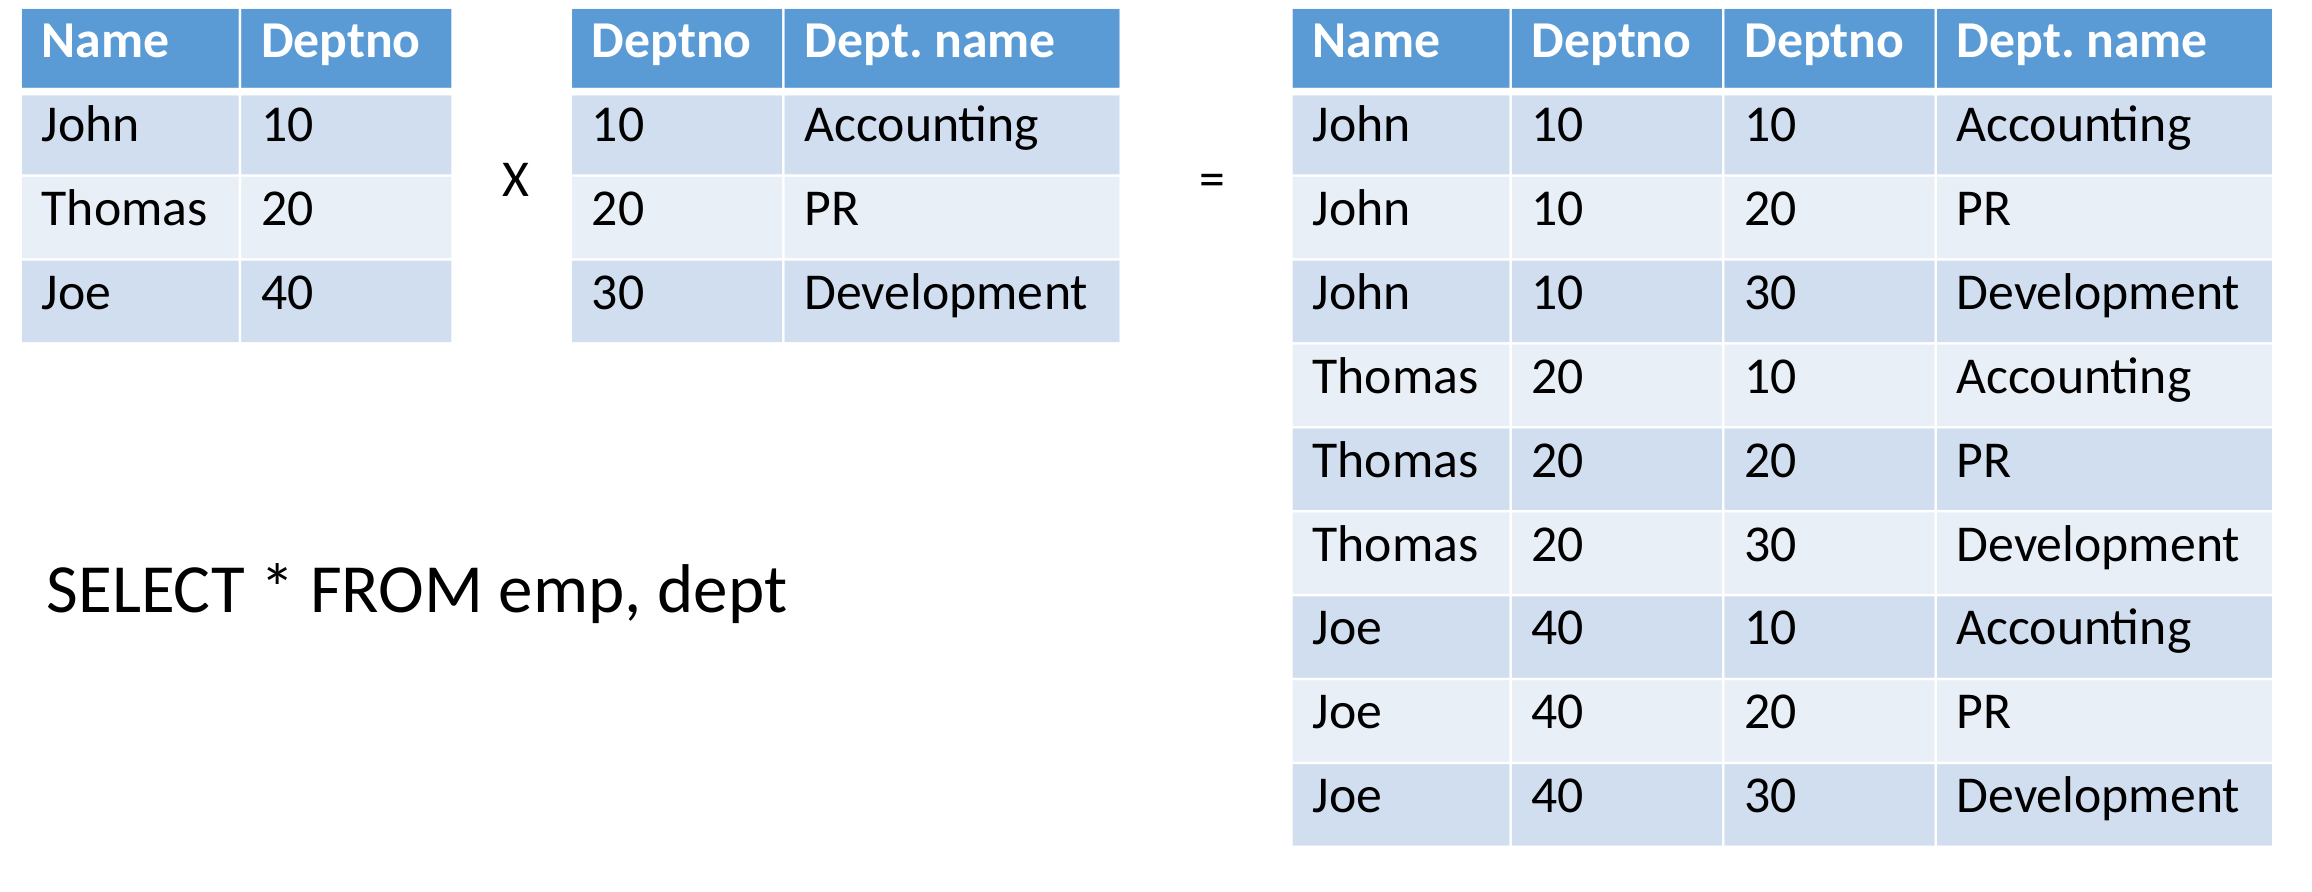
\includegraphics[scale=.12]{join1}
\end{frame}

\begin{frame}{Join --- INNER JOIN}
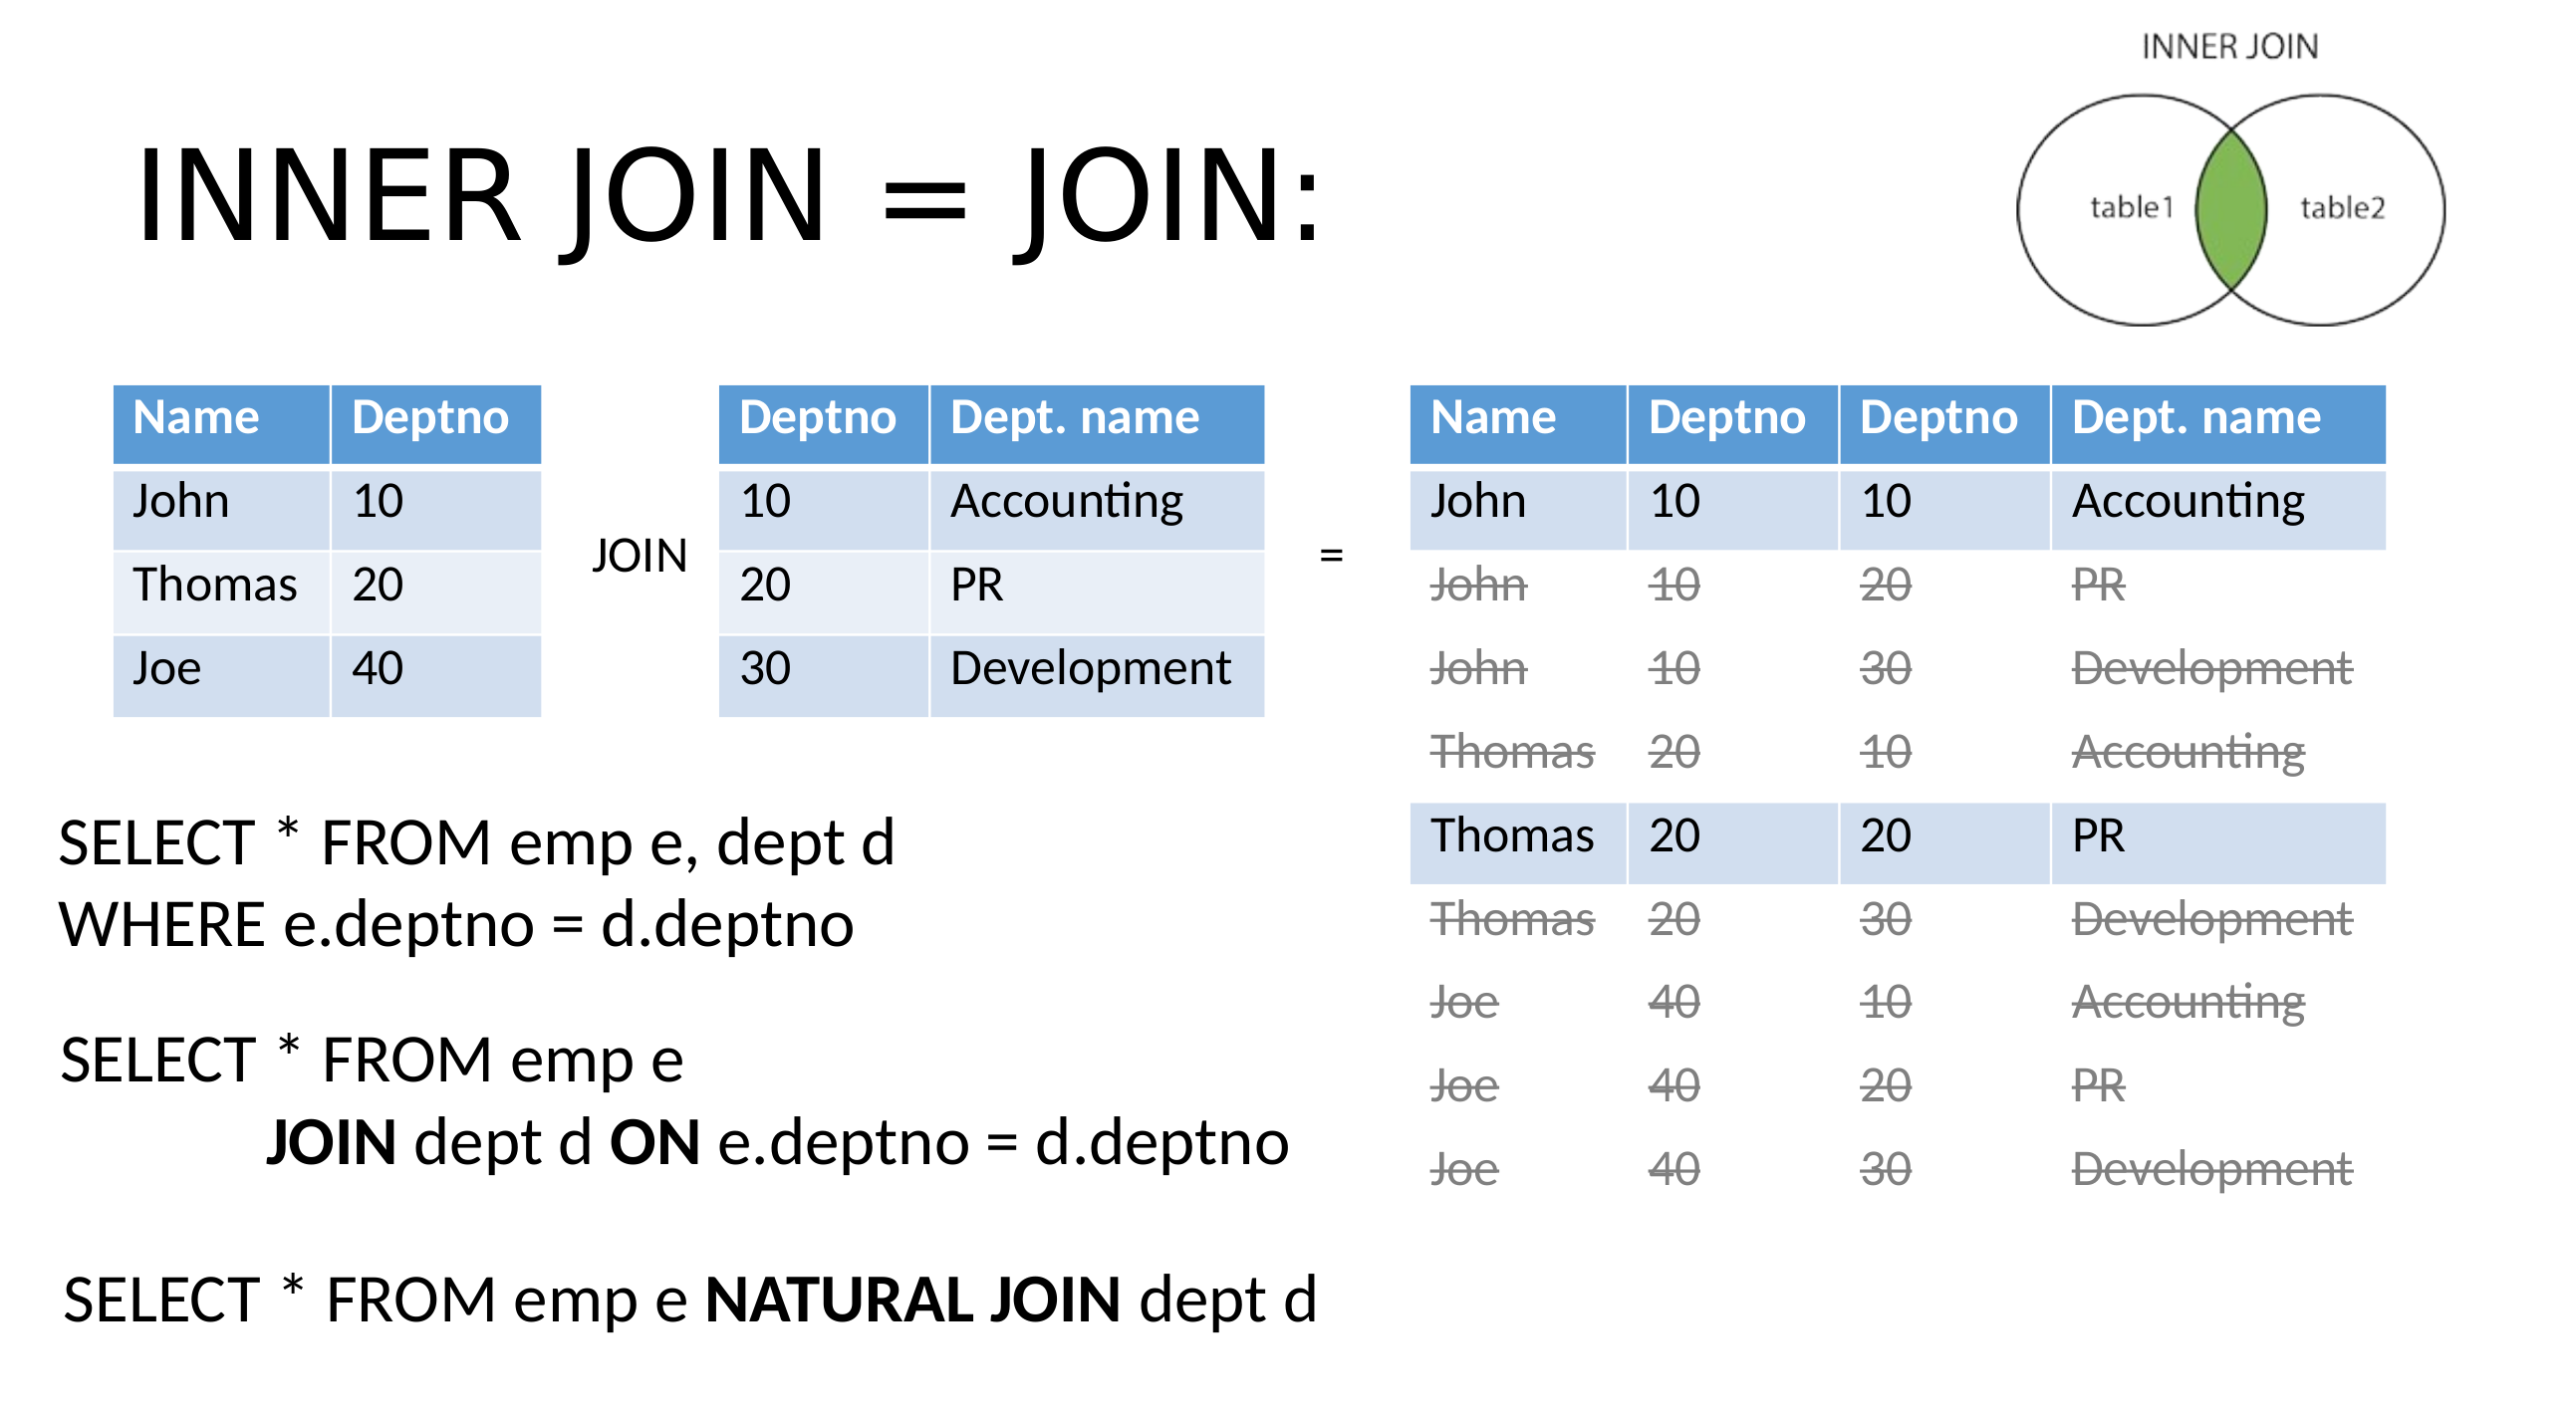
\includegraphics[scale=.12]{join2}
\end{frame}

\begin{frame}{Join --- LEFT JOIN}
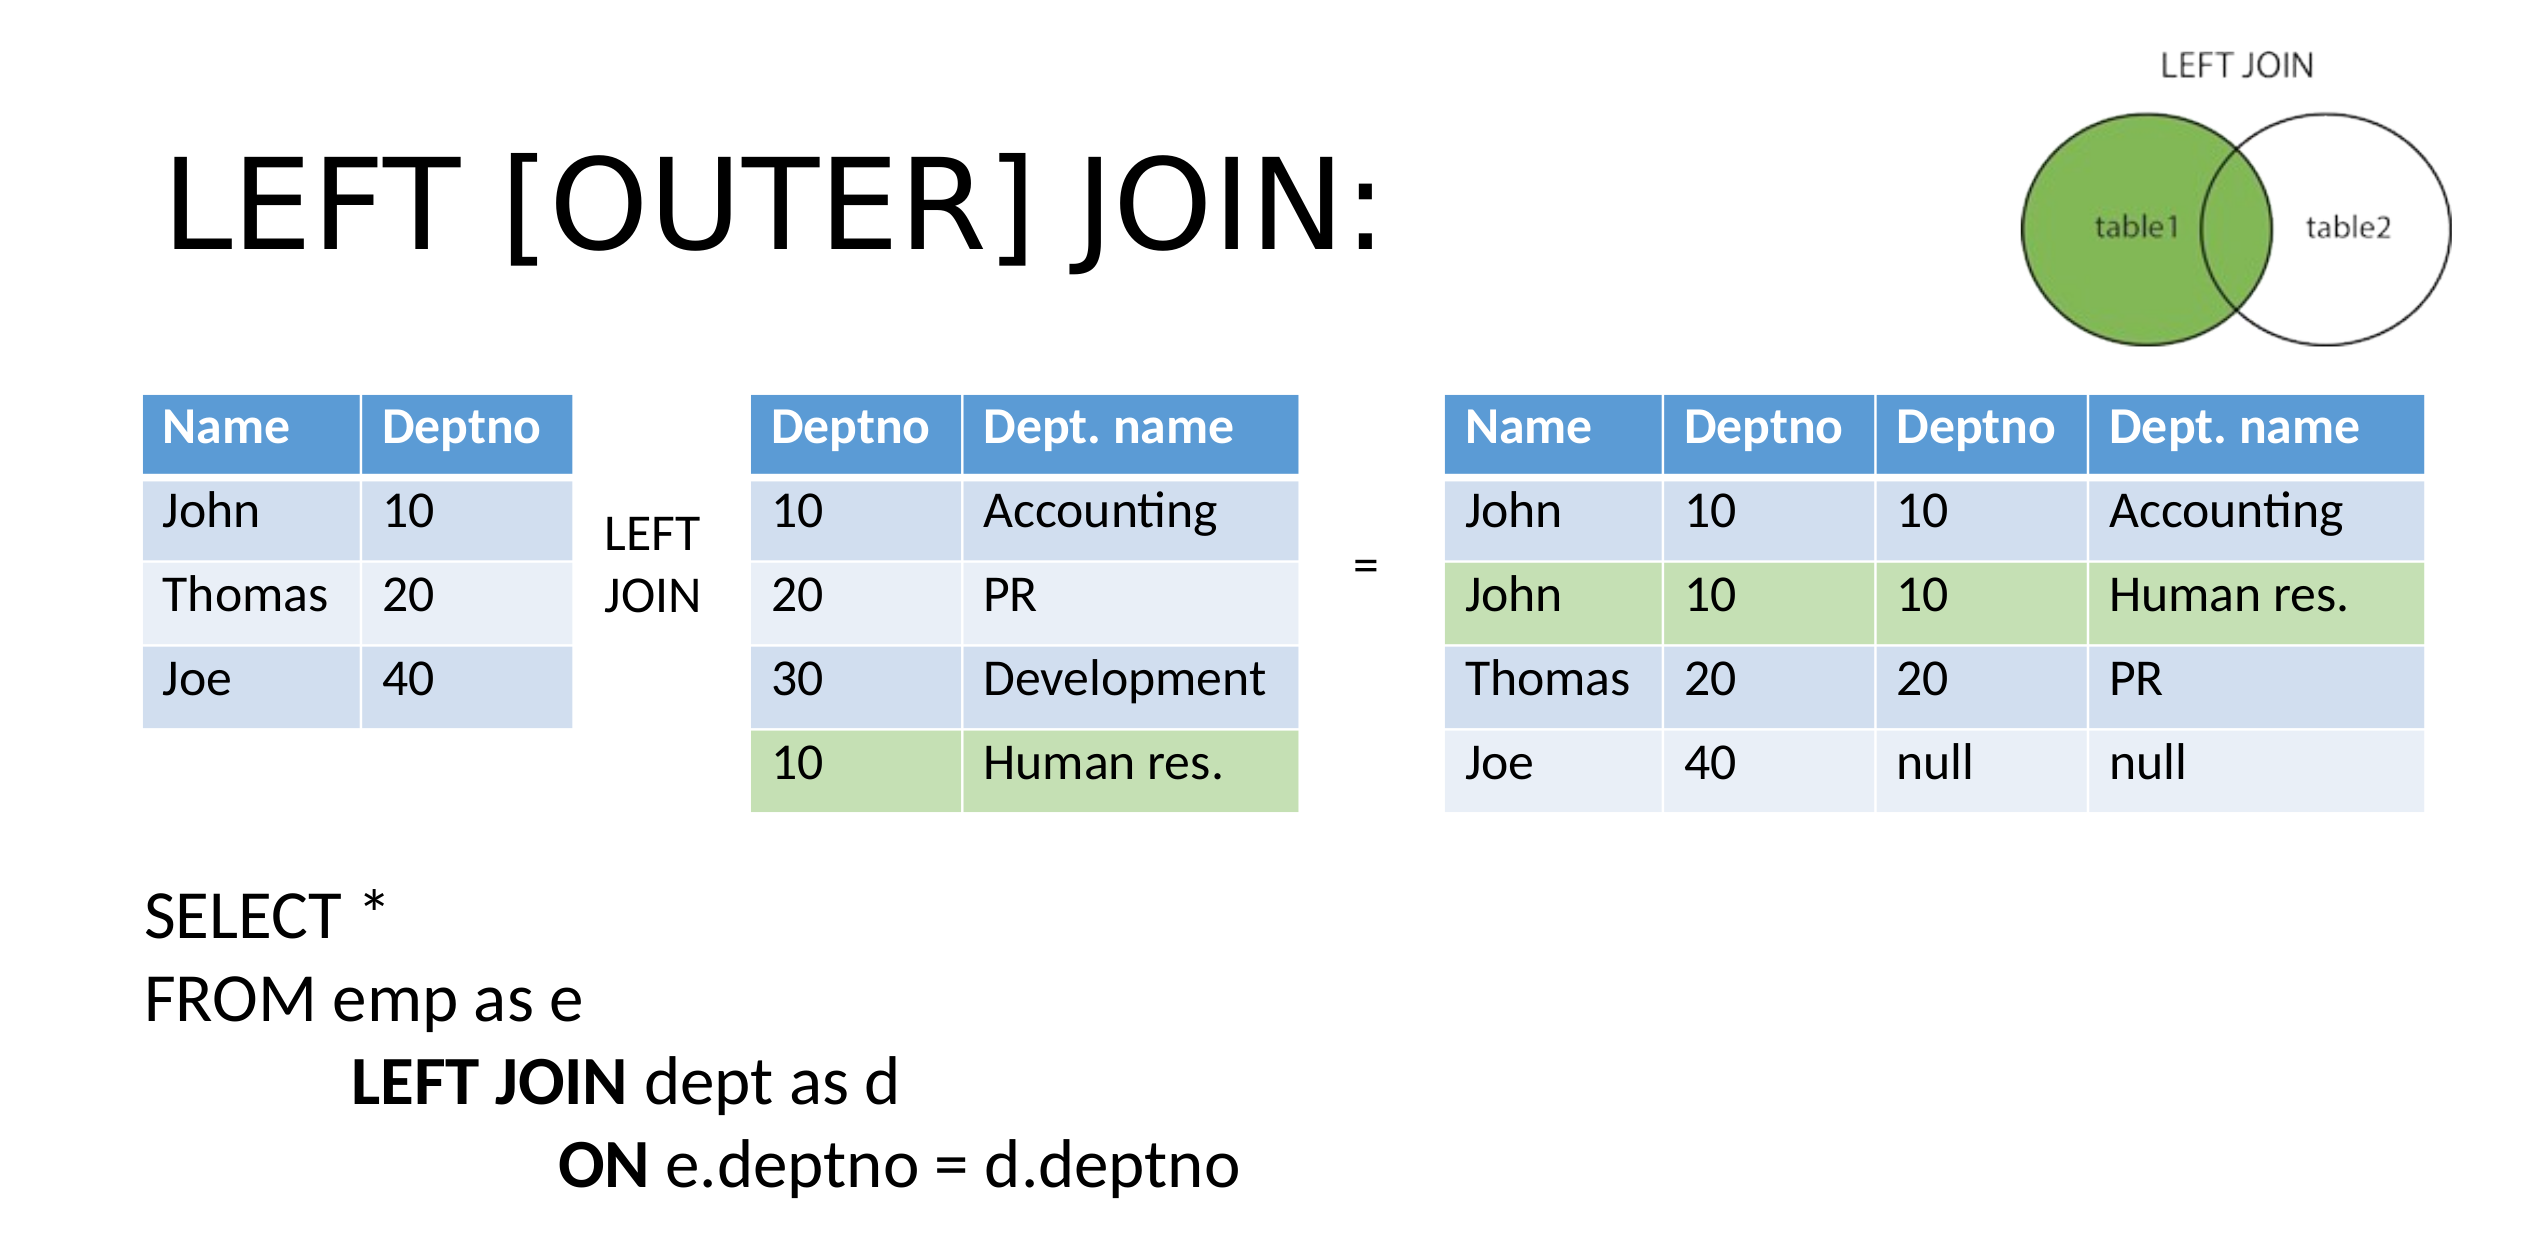
\includegraphics[scale=.12]{join3}
\end{frame}

\begin{frame}{Join --- RIGHT JOIN}
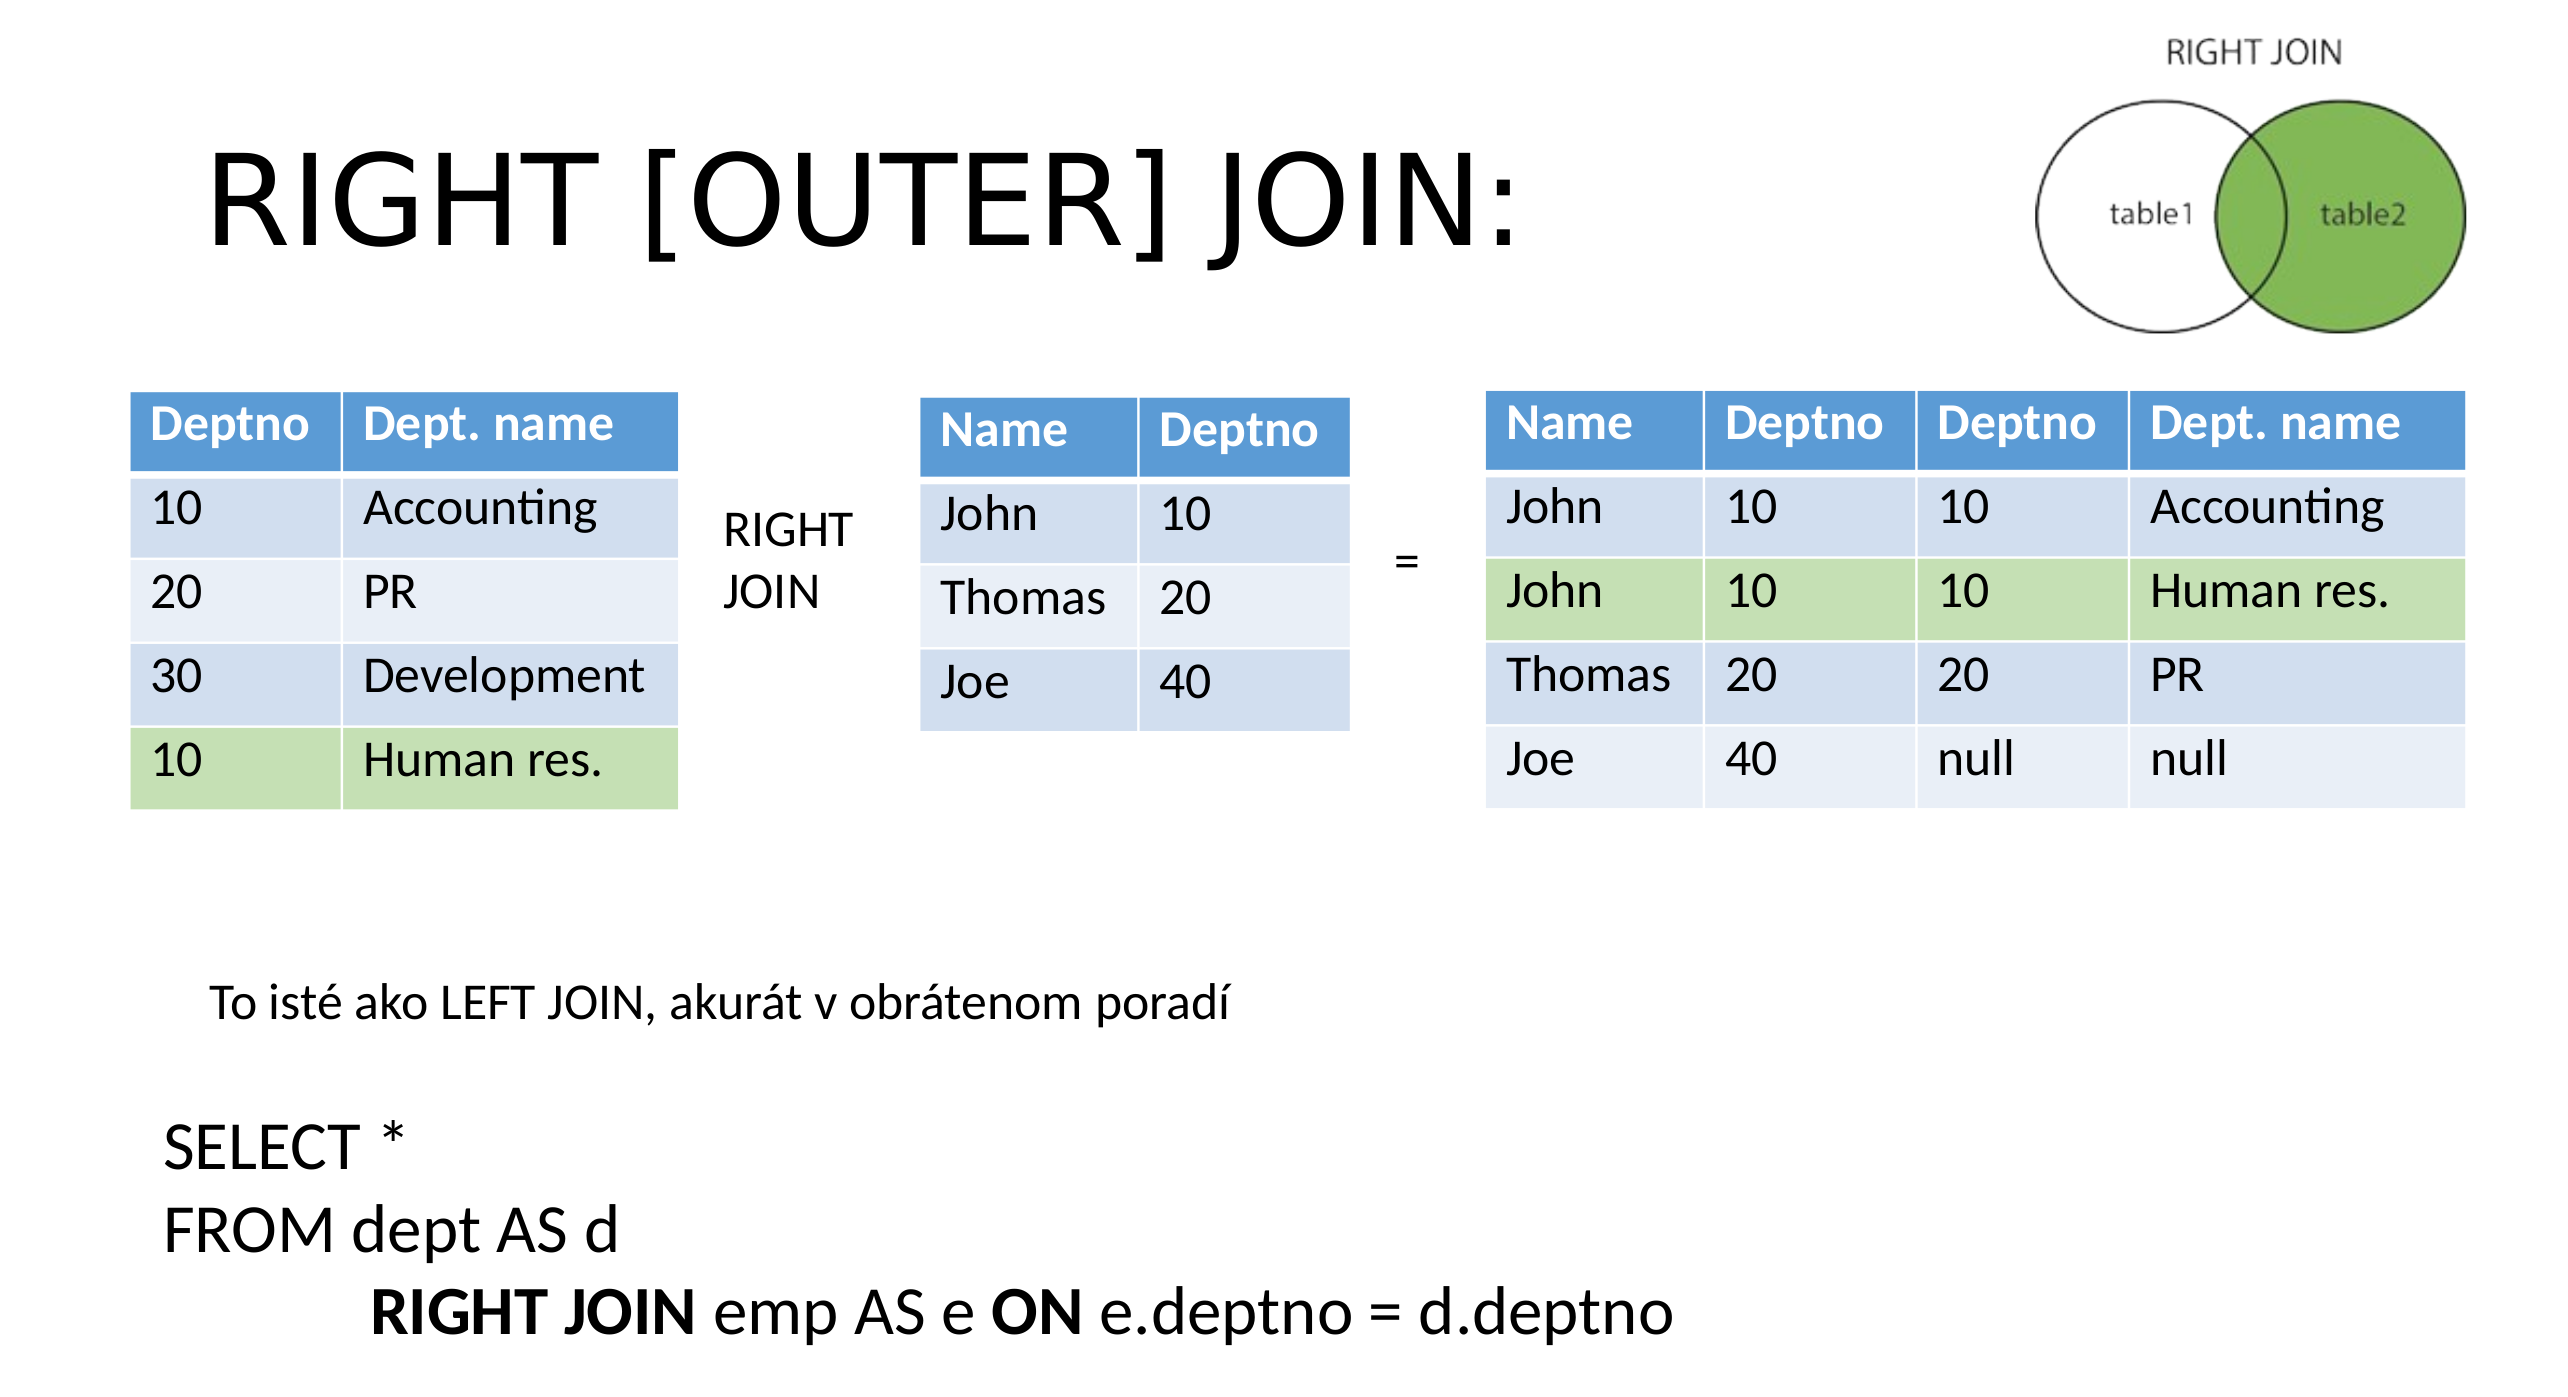
\includegraphics[scale=.12]{join4}
\end{frame}

\begin{frame}{Join --- FULL OUTER JOIN}
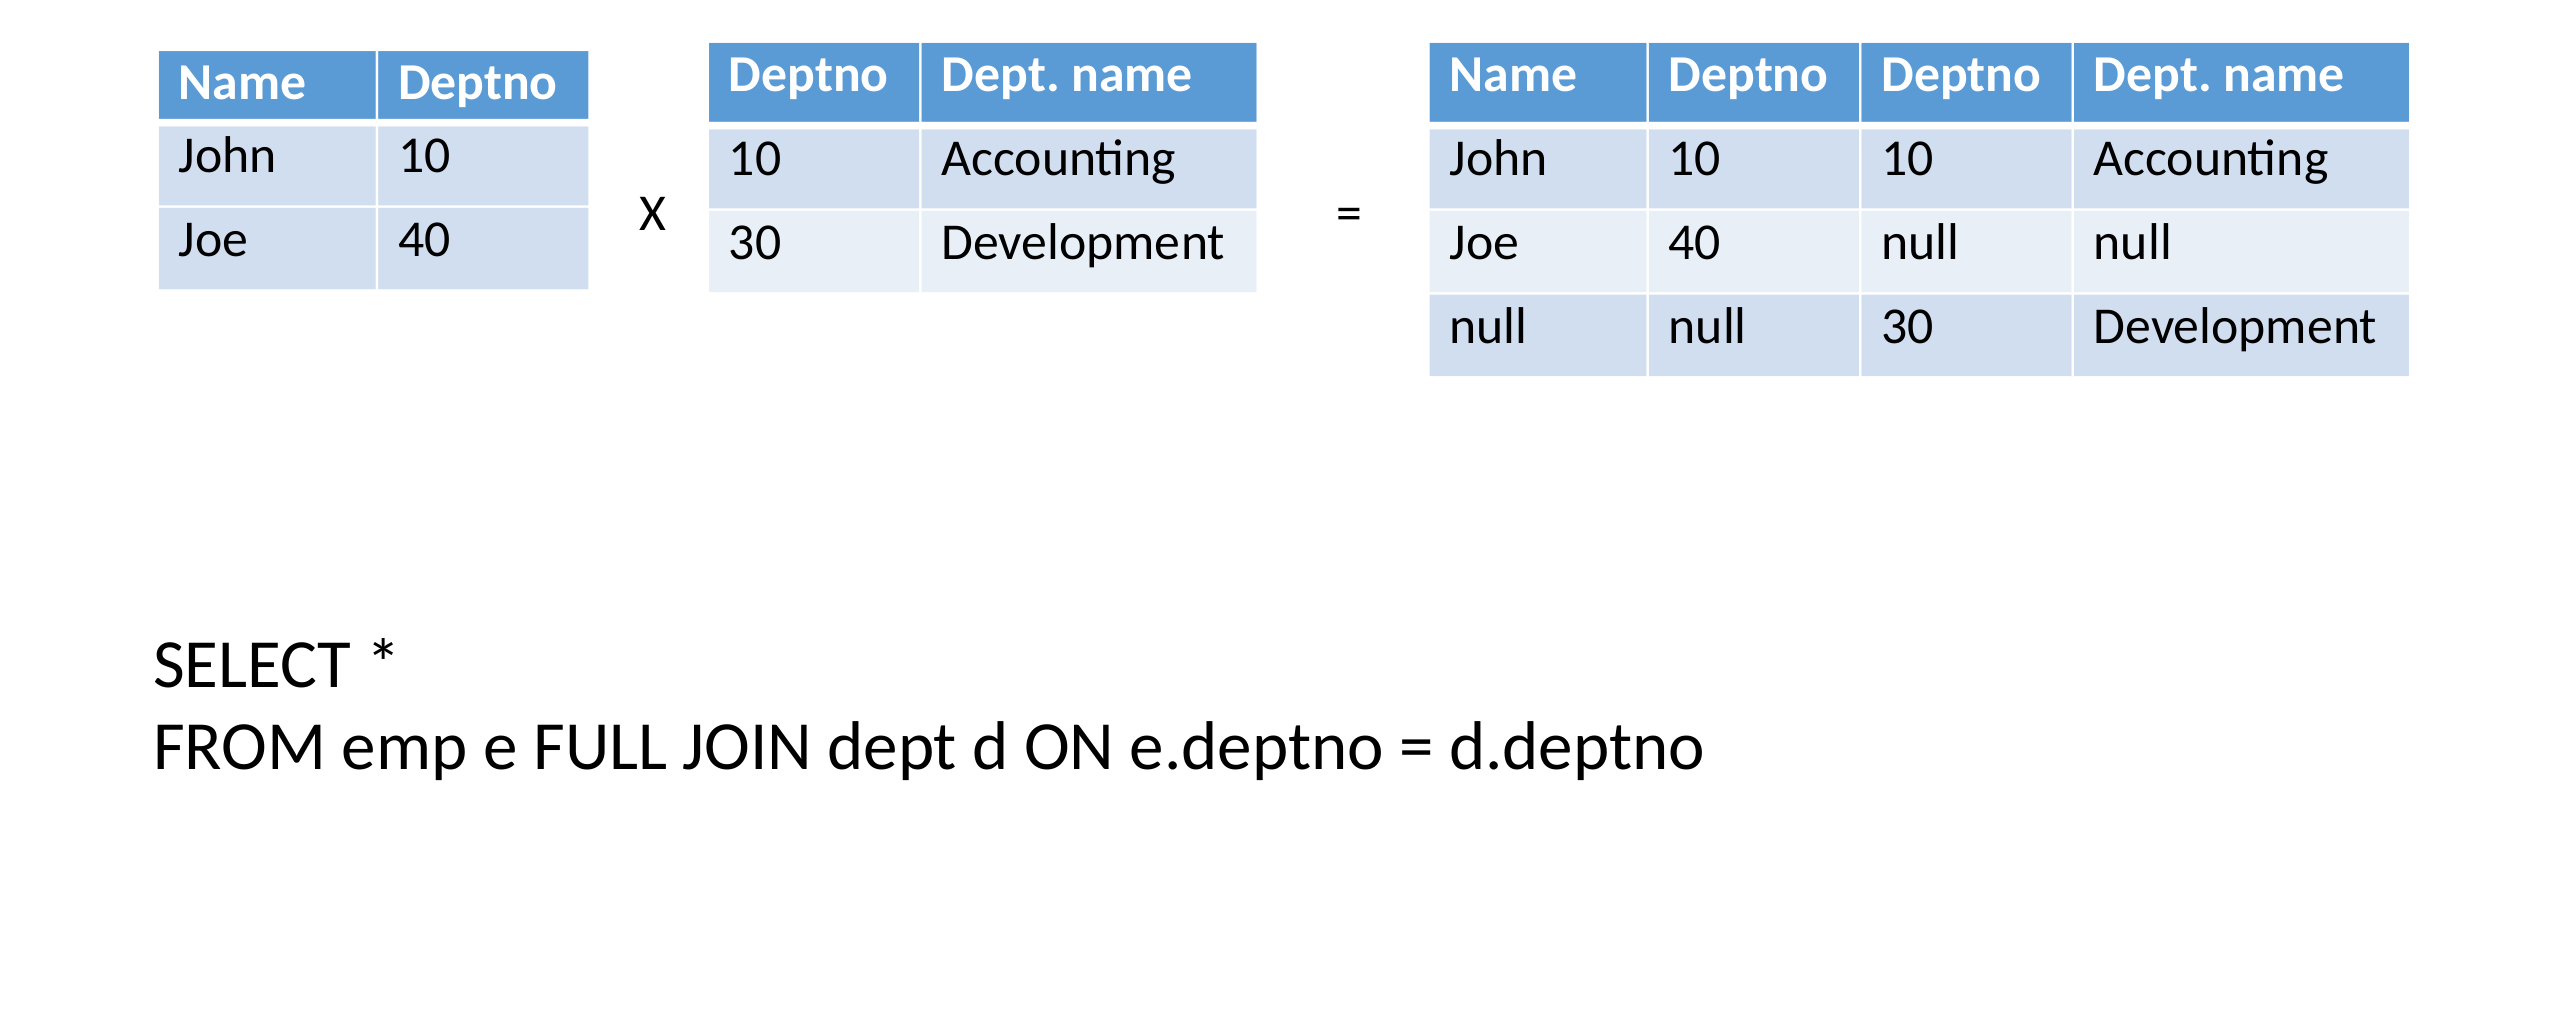
\includegraphics[scale=.12]{join5}
\end{frame}

\begin{frame}[fragile]{Negácia}
Negáciu možno vyjadriť pomocou vnoreného dotazu (subquery) a NOT EXISTS:
\begin{verbatim}
SELECT e.name
FROM emp e
WHERE NOT EXISTS (SELECT 1
                  FROM emp e2 
                  WHERE e2.salary > e.salary)
\end{verbatim}
(Nezáleží na tom, ktoré stĺpce sú vymenované za SELECT vo vnútornom dotaze, pretože EXISTS len testuje, či sa tam nachádza aspoň jeden riadok.)
\end{frame}



\begin{frame}{Literatúra}
\begin{itemize}
\item {\scriptsize\url{https://cs186berkeley.net/notes/note1/}}
\item {\scriptsize\url{https://cs186berkeley.net/notes/note2/}}
\item {\scriptsize\url{https://www.postgresql.org/docs/current/functions-comparison.html}}
\item {\scriptsize\url{https://drive.google.com/file/d/1HCq2KMZ05UvtXGe1nTqNmkwhc3X-NLI3/view}}
\end{itemize}
\end{frame}


\begin{frame}{Úlohy: SQL}
Databáza: \emph{osoba}(A), \emph{pozna}(Kto, Koho)
\begin{itemize}
    \item osoby, ktoré poznajú sysľa
    \item osoby, ktoré majú aspoň dvoch známych (osoby)
    \item osoby, ktoré nepoznajú nikoho (žiadne iné osoby)
    \item osoby, ktoré pozná presne jedna osoba
    \item osoby, ktoré poznajú iba Jožka
    \item osoby, ktoré poznajú všetkých známych svojich známych
    \item osoby, ktoré majú všetky vzťahy symetrické
\end{itemize}
\end{frame}


\end{document}


